\section{Design}
\label{sec: design}

To achieve fast analytics of massive datasets spread over the wide area, we have implemented several key components as part of Meteor, as described below.

\subsection{Location-Aware Map}

\begin{figure}[!ht]
\centering\includegraphics[width=0.5\columnwidth]{figs/lam.pdf}
\vspace{-1.2em}
\caption{Scheduler keeps separate task queues for each cluster/host in location-aware map.}
\label{fig:lam}
\vspace{.7em}
\end{figure}

The system should reduce reliance on network bandwidth since it's a scarce resource. To prevent backhauling
all the data from every location to a centralized location at the beginning of the job, input data should remain in place. To prevent map inputs shuttled over the wire, we implement Location-Aware Map (LAM). LAM scheduling achieves data locality by essentially forbidding a node executing a map task over a data partition residing in a remote cluster. Conceptually LAM scheduling is shown in Figure \ref{fig:lam}. Instead of a FIFO queue of tasks, the scheduler has a separate task queue for each cluster $n$. Therefore a node in cluster $n$ executes a map task that
belonged to its own queue. We provide an API call in Spark to let the programmer attach each data source, i.e. RDD, to a set of nodes. The scheduler puts each map task for partitions for this data source in the appropriate queue. It is interesting to note that Location-Aware Map is equivalent to Delay-Scheduling \cite{delay-scheduling} with infinite delay.
We show in \S \ref{sec:eval}  that LAM provides significant latency and bandwidth improvements over vanilla Spark/MapReduce. 

\subsection{Bandwidth-Aware Work Stealing}

Datasets in the wild are split equally; in fact, there's is a lot of skew in the size of geographically dispersed datasets.  With strict data locality, this will result in some set of clusters rendered idle after finishing their local computation, and hence opportunities for parallelism will go amiss.  Careful scheduling of tasks on remote nodes in this case could lead to even better runtime results. To this end, we implement an adaptive work-stealing policy based on the measured bandwidth between clusters as part of the Spark scheduler. We call this Bandwidth-Aware Work Stealing (BAWS). BAWS scheduling is shown in Figure \ref{fig:baws}. BAWS is implemented on top of LAM. During the LAM stage, all nodes operate in normal. When a node $n$'s task queue gets empty,
instead of remaining idle, it tries to steal a task off a remote node's queue with probability $p$. $p$ is configurable by the user. This work-stealing is bandwidth-aware since the candidate node to steal from is the one that the stealer has the highest measured bandwidth at that time. Therefore BAWS is adaptive to network conditions. 
We show in \S \ref{sec:eval}  that BAWS improves LAM scheduling in terms of job latency.

\begin{figure}[!ht]
\centering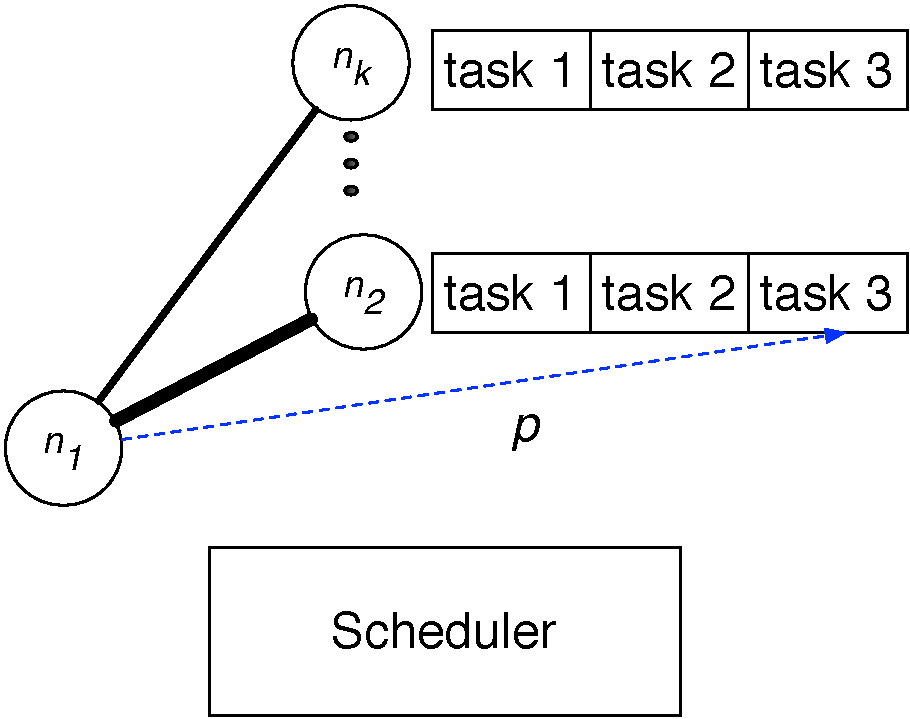
\includegraphics[width=0.5\columnwidth]{figs/BOSS.pdf}
\vspace{-1.2em}
\caption{As part of Bandwidth-Aware Work Stealing, Meteor constantly measures the available bandwidth between each pair of clusters. Work Stealing only kicks in when a node's task queue is empty. It then steals a remote node's task with the highest bandwidth with probability $p$. }
\label{fig:baws}
\vspace{.7em}
\end{figure}

\subsection{Communication-avoiding iterative MapReduce}

There has been a great deal of research on improving iterative MapReduce jobs \cite{haloop, twister, rdd}. by maintaining intermediate data in memory, and consistently partitioning data across iterations. We explore in details how these optimizations help reduce communication in the case of PageRank in section \ref{sec:pagerank}.

Further to these techniques, combiners help reduce inter-node communication \cite{hop}. Combiner work in the same way as reduce functions, but are used in intermediate stages of a MapReduce job in order to summarize input values it was passed for a given key. Combiners essentially perform aggreagation on the map side in order to reduce the amount of network traffic required between map and reduce phases. 

Beyond consistend partitioning, and combining, we wanted to see if \emph{more} could be done to minimize network traffic, potentially at the expense of result correctness. The idea of providing a Òquick and dirtyÓ result over a slow but correct answer has been explored in a few works \cite{blinkdb, hop}, but not necessarily in the context of globally distributed data centers.

Our approach is simple. Assuming we are computing an iterative MapReduce job on a partitionned data set which is consistently partitionned across iterations, we simply periodically avoid sending inter-node updates at the expense of result accuracy. The dataflow diagram is shown in Figure \ref{fig:comm_avoiding}. The datasets at each stage of the algorithm are represented by a dotted line, while the partitions are shown as shaded rectangles. Every time a reduce happens, the nodes have to communicate with one-another in order to update their respective key values. This communication can be expensive, and depending on the partitioning of the input dataset, and the dependencies between those datasets, could require high-bandwidth. 

\begin{figure}[!ht]
\centering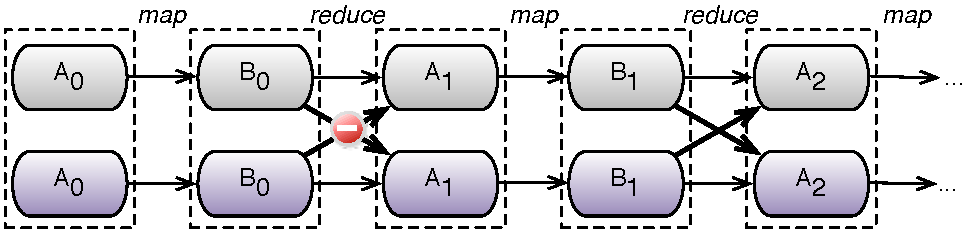
\includegraphics[width=0.9\columnwidth]{figs/comm_avoiding.pdf}
\caption{For iterative MapReduce jobs, Meteor can periodically avoid all-to-all communication. This technique can be used to respond to bandwidth fluctuations, at the cost of result convergence.}
\label{fig:baws}
\vspace{.7em}
\end{figure}